\setlength{\doublerulesep}{0.3pt}

\themaN
\graphicspath{{../../S11_Multiples_et_diviseurs/Images/}}

\chapter{Multiples et diviseurs}
\label{S11}


%%%%%%%%%%%%%%%%%%%%%%%%%%%%%%%%%%%%%%%%%%
%%%%%%%%%%%%%%%%%%%%%%%%%%%%%%%%%%%%%%%%%%
\begin{prerequis}[Connaissances $\heartsuit$ et compétences $\diamondsuit$ du cycle 4]
   \begin{itemize}
      \item Multiples et diviseurs.
      \item Critères de divisibilité par 2, 3, 5, 9.
      \item Division euclidienne.
      \item[\com] Déterminer si un entier est ou n'est pas multiple ou diviseur d'un autre entier.
      \item[\com] Utiliser un critère de divisibilité par 2, 3, 5, 9, 10.
      \item[\com] Modéliser et résoudre des problèmes mettant en jeu la divisibilité.
   \end{itemize}
\end{prerequis}

\vfill

\begin{debat}[Débat : la division euclidienne] 
   Le nom de {\bf division euclidienne} est un hommage rendu à {\it Euclide} (300 av. J.-C.), mathématicien grec qui en explique le principe par soustractions successives dans son \oe uvre {\it Les éléments}. Mais elle apparait très tôt dans l'histoire des mathématiques, par exemple dans les mathématiques égyptiennes, babyloniennes et chinoises.
   \begin{center}
      \begin{pspicture}(0,1)(4,4.5)
         \psline[linewidth=1mm](2,1)(2,4)
         \psline[linewidth=1mm](2,3)(4,3)
         \textcolor{B1}{\it\large
         \rput(0.8,3.5){dividende}
         \rput(3,3.5){diviseur}
         \rput(3,2.5){quotient}
         \rput(3,2){\small (euclidien)}
         \rput(1,1.5){reste}}
      \end{pspicture}
   \end{center}
   \bigskip
   \begin{cadre}[B2][F4]
      \begin{center}
         Vidéo : \href{https://www.youtube.com/watch?v=VWS9NyXbEyY&t=18s}{\bf Division euclidienne avec matériel multibase}, chaîne YouTube {\it Méthode Heuristique}.
      \end{center}
   \end{cadre}
\end{debat}

\vfill

\textcolor{PartieGeometrie}{\sffamily\bfseries Cahier de compétences} : $\varnothing$


%%%%%%%%%%%%%%%%%%%%%%%%%%%%%%%%%%
%%%%%%%%%%%%%%%%%%%%%%%%%%%%%%%%%%
\activites

\begin{activite}[Les multiplications incomplètes]
   {\bf Objectifs} : calculer mentalement des multiplications et des divisions ; résoudre un problème de calcul mental ; compléter un tableau à double entrée.
   \begin{QCM}
   Compléter ces tables de multiplication dont on a effacé le contenu de certaines cases. Les nombres sont tous strictement positifs, il ne peut pas y avoir deux fois le même nombre sur une même colonne ou une même ligne. \medskip
   {\hautab{1.82}
   \partie[piste verte] \medskip
      \hfill
      \begin{tabular}{|C{0.5}||C{0.5}|C{0.5}|}
         \hline
         {\Large $\times$} & & \\
         \hline\hline
         & & 24 \\
         \hline
         & 25 & 30 \\
         \hline
      \end{tabular}
      \hfill
      \begin{tabular}{|C{0.5}||C{0.5}|C{0.5}|}
         \hline
         {\Large $\times$} & & 7 \\
         \hline\hline
         & & 21 \\
         \hline
         4 & 8 & \\
         \hline
      \end{tabular}
      \hfill
      \begin{tabular}{|C{0.5}||C{0.5}|C{0.5}|}
         \hline
         {\Large $\times$} & 6 & \\
         \hline\hline
         & 24 & 32 \\
         \hline
         & 36 & \\
         \hline
      \end{tabular}
      \hfill
      \begin{tabular}{|C{0.5}||C{0.5}|C{0.5}|}
         \hline
         {\Large $\times$} & 3 & \\
         \hline\hline
         & & 18 \\
         \hline
         5 & & 45 \\
         \hline
      \end{tabular}
      \hspace*{1cm} \\
         
   \partie[piste bleue] \medskip
      \hfill
      \begin{tabular}{|C{0.5}||C{0.5}|C{0.5}|C{0.5}|}
         \hline
         {\Large $\times$} & 2 & & \\
         \hline\hline
         & & 9 & \\
         \hline
         & 8 & & \\
         \hline
         & 16 & & 56 \\
         \hline
      \end{tabular}
      \hfill
      \begin{tabular}{|C{0.5}||C{0.5}|C{0.5}|C{0.5}|}
         \hline
         {\Large $\times$} & 2 & & \\
         \hline\hline
         4 & & 16 & \\
          \hline
         & & & 35 \\
         \hline
         9 & 18 & & 45 \\
         \hline
      \end{tabular}
      \hfill
      \begin{tabular}{|C{0.5}||C{0.5}|C{0.5}|C{0.5}|}
         \hline
         {\Large $\times$} & & 7 & \\
         \hline\hline
         & 12 & & 32 \\
         \hline
         & & & 64 \\
         \hline
         & & 63 & 72 \\
         \hline
      \end{tabular}
      \hspace*{1cm} \\
      
   \partie[piste rouge] \medskip 
      \hfill
      \begin{tabular}{|C{0.5}||C{0.5}|C{0.5}|C{0.5}|}
         \hline
         {\Large $\times$} & & 3 & \\
         \hline\hline
         & 20 & & \\
         \hline
         & & 18 & \\
         \hline
         & & 6 & 4 \\
         \hline
      \end{tabular}
      \hfill
      \begin{tabular}{|C{0.5}||C{0.5}|C{0.5}|C{0.5}|}
         \hline
         {\Large $\times$} & & & 7 \\
         \hline\hline
         2 & & & 14 \\
         \hline
         & 72 & 54 & \\
          \hline
         & 40 & & 35 \\
         \hline
      \end{tabular}
      \hfill
      \begin{tabular}{|C{0.5}||C{0.5}|C{0.5}|C{0.5}|}
         \hline
         {\Large $\times$} & & & \\
         \hline\hline
         & 18 & & 15 \\
         \hline
         & & 64 & \\
         \hline
         & & 32 & \\
         \hline
      \end{tabular}
      \hspace*{1cm} \\
      
   \partie[piste noire] \medskip
      \hfill
      \begin{tabular}{|C{0.5}||C{0.5}|C{0.5}|C{0.5}|}
         \hline
         {\Large $\times$} & & & 10 \\
         \hline\hline
         & 20 & 8 & \\
         \hline
         & 35 & & 70 \\
         \hline
         & & & 100 \\
         \hline
      \end{tabular}
      \hfill
      \begin{tabular}{|C{0.5}||C{0.5}|C{0.5}|C{0.5}|}
         \hline
         {\Large $\times$} & & & \\
         \hline\hline
         & & 45 & \\
         \hline
         & 28 & & \\
         \hline
         & 44 & & 99 \\
         \hline
      \end{tabular}
      \hfill
      \begin{tabular}{|C{0.5}||C{0.5}|C{0.5}|C{0.5}|}
         \hline
         {\Large $\times$} & & 13 & \\
         \hline\hline
         & & 65 & \\
         \hline
         & 42 & & 49 \\
         \hline
         & 72 & & 84 \\
         \hline
      \end{tabular}}
      \hspace*{1cm}
      \vspace*{1cm}
   \end{QCM}
\end{activite}


%%%%%%%%%%%%%%%%%%%%%%%%%%%%%%%%%%%%%%%%%%
%%%%%%%%%%%%%%%%%%%%%%%%%%%%%%%%%%%%%%%%%%
\cours 

%%%%%%%%%%%%%%%%%%%%%%%%%%
\section{Multiples et diviseurs}

\begin{minipage}{10cm}
   {\it Rappel :} effectuer une division euclidienne d'un {\bf dividende} $a$ par un {\bf diviseur} $b$, c'est trouver deux entiers appelés {\bf quotient} $q$ et {\bf reste} $r$ tels que $a=b\times q+r$ où $r<b$. \\
   Dans l'exemple ci-contre, on peut écrire : $123 =5\times24+3$.
\end{minipage}
\qquad
\begin{minipage}{4cm}
   \begin{pspicture}(-0.5,-0.5)(4,3)
      \rput(1,1.2){$\opidiv[displayintermediary=all,voperation=top]{123}{5}$}
      \psline[linecolor=A1]{->}(0.7,2.8)(0.7,2.4)
      \rput(0.7,3){\textcolor{A1}{dividende}}
      \psline[linecolor=A1]{<-}(1.9,2.3)(2.4,2.3)
      \rput[l](2.5,2.3){\textcolor{A1}{diviseur}}
      \psline[linecolor=B1]{<-}(2.2,1.7)(2.7,1.7)
      \rput[l](2.8,1.7){\textcolor{B1}{quotient}}
      \psline[linecolor=B1]{<-}(1.4,0.2)(1.9,0.2)
      \rput[l](2,0.2){\textcolor{B1}{reste}}
   \end{pspicture}
\end{minipage}

\begin{definition}
   $a$ et $b$ sont deux nombres entiers. Lorsque le reste de la division de $a$ par $b$ est égal à 0, on dit que $a$ est un \textbf{multiple} de $b$, ou que $b$ est un \textbf{diviseur} de $a$, ou encore que $a$ est \textbf{divisible} par $b$.
\end{definition}

\begin{exemple*1}
   \begin{itemize}
      \item 15 est un multiple de 3 car $15=3\times 5+\textcolor{A1}{0}$, on peut aussi dire que 3 est un diviseur de 15, ou que 15 est divisible par 3.
      \item 17 n'est pas un multiple de 3 car $17=3\times 5+\textcolor{A1}{2}$.
      \item Les diviseurs de 24 sont 1; 2; 3; 4; 6; 8; 12 et 24.
      \item Il y a une infinité de multiples de 18, comme par exemple 18 ; 36 ; 54 ; 180\dots
   \end{itemize}
   \vspace*{-3mm}
\end{exemple*1}

%%%%%%%%%%%%%%%%%%%%%%%%%%
\section{Critères de divisibilité}

\begin{propriete}
   \begin{itemize}
      \item un nombre est divisible par 2 s'il se termine par 0 ; 2 ; 4 ; 6 ou 8 ;
      \item un nombre est divisible par 3 si la somme de ses chiffres est un multiple de 3 ;
      \item un nombre est divisible par 5 s'il se termine par 0 ou 5 ;
      \item un nombre est divisible par 9 si la somme de ses chiffres est un multiple de 9 ;
      \item un nombre est divisible par 10 s'il se termine par 0.
   \end{itemize}
   \vspace*{-3mm}
\end{propriete}

\begin{exemple*1}
   \begin{itemize}
      \item 252 et 253 sont-ils divisibles par 3 ?
      \item 52\,362 et 52\,363 sont-ils divisibles par 9 ?
    \end{itemize}   
   \correction
      \begin{itemize}
         \item $2+5+2=9$ est multiple de 3 donc, 252 est divisible par 3. \\
            $2+5+3=10$ n'est pas multiple de 3 donc, 253 n'est pas divisible par 3.
         \item $5+2+3+6+2=18$ est multiple de 9 donc, 52\,362 est divisible par 9, et donc par 3. \\
            $5+2+3+6+3=19$ n'est pas multiple de 9 donc, 52\,363 n'est pas divisible par 9.
       \end{itemize}
    \vspace*{-3mm}
\end{exemple*1}

\begin{remarque}
   pour savoir si un nombre est divisible par $3$, on peut calculer la somme des chiffres du nombre obtenu jusqu'à ce que l'on trouve un seul chiffre : \\
   pour $563\,387\,981$, on calcule : $5+6+3+3+8+7+9+8+1=50$. Puis on calcule $5+0=5$.
   $5$ n'est pas divisible par $3$ donc, $563\,387\,981$ n'est pas divisible par $3$.
\end{remarque}



%%%%%%%%%%%%%%%%%%%%%%%%%%%%%%%%%%%%%
%%%%%%%%%%%%%%%%%%%%%%%%%%%%%%%%%%%%%
\exercicesbase

\begin{colonne*exercice}

\serie{Division euclidienne} %%%

\bigskip

\begin{exercice} %1
   Effectuer la division euclidienne de 307 par 7 puis de 13\,758 par 25.
\end{exercice}
        
\begin{corrige}
   {\small \opidiv[displayintermediary=all,voperation=top]{307}{7} \qquad \opidiv[displayintermediary=all,voperation=top]{13758}{25}} \\
   {\blue $307 =7\times43+6$} et {\blue $13\,758 =25\times550+8$}.
\end{corrige}

\bigskip


\begin{exercice} %2
   On donne les égalités : \\
   $415 = 7\times59+2$ \; et \; $56\times57 = 3\,192$. \\
   Sans effectuer de calculs, donner le quotient et le reste des divisions euclidiennes suivantes.
   \begin{colenumerate}{2}
      \item 415 par 7
      \item 3\,192 par 56
      \item 415 par 59
      \item 3\,192 par 57
   \end{colenumerate}
\end{exercice}

\begin{corrige}
   \ \\ [-5mm]
   \begin{enumerate}
      \item Le quotient de 415 par 7 est {\blue 59}, le reste est {\blue 2}.
      \item Le quotient de 3\,192 par 56 est {\blue 57}, le reste est {\blue 0}.
      \item Le quotient de 415 par 59 est {\blue 7}, le reste est {\blue 2}.
      \item Le quotient de 3\,192 par 57 est {\blue 56}, le reste est {\blue 0}.
   \end{enumerate}
\end{corrige}

\bigskip


\begin{exercice} %3
   Résoudre les problèmes suivants :
   \begin{enumerate}
      \item 6\,798 supporters d'un club de rugby doivent faire un déplacement en car pour soutenir leur équipe. Chaque car dispose de 55 places. Combien de cars faut-il réserver ?
      \item Des stylos sont conditionnés par boîte de 40. Jules a 2\,647 stylos. Combien lui en manque-t-il pour avoir des boîtes entièrement remplies ?
      \item Trois amis participent à une chasse au trésor et trouvent 1\,419 pièces en chocolat. Si le partage est équitable, combien de pièces en chocolat auront-ils chacun ? Zakaria arrive et leur rappelle que c'est lui qui leur a prêté sa boussole. Il exige donc d'avoir la même part que chacun des trois autres plus les pièces restantes. Combien de pièces recevra-t-il ?
   \end{enumerate}
\end{exercice}

\begin{corrige}
   \ \\ [-5mm]
   \begin{enumerate}
      \item On effectue la division : {\small \opidiv[displayintermediary=all,voperation=top]{6798}{55}} \\
         Il faudra donc réserver {\blue 124 cars}.
      \item On effectue la division : {\small \opidiv[displayintermediary=all,voperation=top]{2647}{40}} \\
         Il lui reste 7 stylos pour une boite de 40, il faut donc ajouter {\blue 33 stylos} pour compléter la boite.
      \item On effectue la division : {\small \opidiv[displayintermediary=all,voperation=top]{1419}{3}} \\
         Chaque ami aura donc {\blue 473 pièces en chocolat}. \\
         Lorsque Zakaria arrive, on fait {\small \opidiv[displayintermediary=all,voperation=top]{1419}{4}} \\
         Il recevra $(354+3)$ pièces en chocolat, soit {\blue 357}.
   \end{enumerate}
\end{corrige}

\bigskip


%%%%%%%%%%%%%%%
\serie{Multiples et diviseurs}

\bigskip

 \begin{exercice} %7
   Trouver tous les diviseurs des nombres suivants : \\
   14 ; 40 ; 48 et 2\,037.
\end{exercice}

\begin{corrige}
   \begin{itemize}
      \item Diviseurs de 14 : {\blue 1 ; 2 ; 7 ; 14}.
      \item Diviseurs de 40 : {\blue 1 ; 2 ; 4 ; 5 ; 8 ; 10 ; 20 ; 40}.
      \item Diviseurs de 48 : {\blue 1 ; 2 ; 3 ; 4 ; 6 ; 8 ; 12 ; 16 ; 24 ; 48}.
      \item Diviseurs de 2\,037 : {\blue 1 ; 3 ; 7 ; 21 ; 97 ; 291 ; 679 ; 2037}.
   \end{itemize}
\end{corrige}

\bigskip


\begin{exercice} %5
   Ecrire :
   \begin{enumerate}
      \item La liste des dix premiers multiples de 6.
      \item Cinq multiples de 11.
      \item Tous les multiples de 13 inférieurs à 80.
      \item Le plus grand multiple de 12 inférieur à 75.
      \item Le plus grand multiple de 36 inférieur à 100.
      \item Le plus petit multiple de 9 supérieur à 1\,200.
      \item Le plus petit multiple de 14 supérieur à 710 ?
      \item Le plus petit et le plus grand diviseur de 2\,021.
   \end{enumerate}
\end{exercice}

\begin{corrige}
   \ \\ [-5mm]\begin{enumerate}
      \item Dix premiers multiples de 6 : \\
         {\blue 0 ; 6 ; 12 ; 18 ; 24 ; 30 ; 36 ; 42 ; 48 ; 54}.
      \item Cinq multiples de 11 : \\
         {\blue 0 ; 11 ; 22 ; 33 ; 44}.
      \item Multiples de 13 inférieurs à 80 : \\
         {\blue 0 ; 13 ; 26 ; 39 ; 52 ; 65 ; 78}
      \item Plus grand multiple de 12 inférieur à 75 : {\blue 72}.
      \item Plus grand multiple de 36 inférieur à 100 : {\blue 72}.
      \item Plus petit multiple de 9 supérieur à 1\,200 : {\blue 1206}.
      \item Plus petit multiple de 14 supérieur à 710 : {\blue 714}.
      \item Plus grand/petit diviseur de 2\,021 : {\blue 1 et 2\,021}.
   \end{enumerate}
\end{corrige}

\bigskip


\begin{exercice} %6
   Répondre aux questions suivantes :
   \begin{enumerate}
      \item 
      \begin{enumerate}
         \item Écrire tous les multiples de 3 inférieurs à 41. 
         \item Écrire tous les multiples de 5 inférieurs à 41.
         \item Entourer les multiples communs à 3 et 5.
         \item Que remarque-t-on ?
      \end{enumerate}
      \item
      \begin{enumerate}      
         \item Écrire tous les multiples de 4 inférieurs à 50. 
         \item Écrire tous les multiples de 6 inférieurs à 50.
         \item Entourer les multiples communs à 4 et 6.
         \item Que remarque-t-on ?
      \end{enumerate}
   \end{enumerate}
\end{exercice}

\begin{corrige}
   \ \\ [-5mm]
   \begin{enumerate}
      \item 
      \begin{enumerate}
         \item Multiples de 3 inférieurs à 41 : \\ \smallskip
            {\blue \fbox{0} ; 3 ; 6 ; 9 ; 12 ; \fbox{15} ; 18 ; 21 ; 24 ; 27 ; \fbox{30} ; 33 ; 36 ; 39} \smallskip
         \item Multiples de 5 inférieurs à 41 : \\ \smallskip
            {\blue \fbox{0} ; 5 ; 10 ; \fbox{15} ; 20 ; 25 ; \fbox{30} ; 35 ; 40} \smallskip
         \item On a entouré : {\blue 0 ; 15 ; 30}.
         \item On remarque que les multiples communs à 3 et à 5 sont les {\blue multiples de 15}.
      \end{enumerate}
      \setcounter{enumi}{1}
      \item
      \begin{enumerate}
         \item Multiples de 4 inférieurs à 50 : \\ \smallskip
            {\blue \fbox{0} ; 4 ; 8 ; \fbox{12} ; 16 ; 20 ; \fbox{24} ; 28 ; 32 ; \fbox{36} ; 40 ; 44 ; \fbox{\!48\!}} \smallskip
         \item Multiples de 6 inférieurs à 50 : \\ \smallskip
            {\blue \fbox{0} ; 6 ; \fbox{12} ; 18 ; \fbox{24} ; 30 ; \fbox{36} ; 42 ; \fbox{48}} \smallskip
         \item On a entouré : {\blue 0 ; 12 ; 24 ; 36 ; 48}.
         \item On remarque que les multiples communs à 4 et à 6 sont les {\blue multiples de 12}.
      \end{enumerate}
   \end{enumerate}
\end{corrige}

\bigskip


%%%%%%%%%%%%
\serie{Critères de divisibilité}

\bigskip

\begin{exercice} %8
   Les nombres 30 ; 27 ; 246 ; 325 ; 4\,238 et 6\,139 sont-ils divisibles par 2 ? par 3 ? par 5 ? par 9 ?
\end{exercice}

\begin{corrige}
   On résume les résultats dans un tableau : \\ \medskip
   {\hautab{1.25}
   \begin{CLtableau}{0.95\linewidth}{7}{c}
      \hline
      & 30 & 27 & 246 & 325 & 4\,238 & 6\,139 \\
      \hline
      par 2 & \textcolor{blue}{$\surd$} & & \textcolor{blue}{$\surd$} & & \textcolor{blue}{$\surd$} & \\
      \hline
      par 3 & \textcolor{blue}{$\surd$} & \textcolor{blue}{$\surd$} & \textcolor{blue}{$\surd$} & & & \\
      \hline
      par 5 & \textcolor{blue}{$\surd$} & & & \textcolor{blue}{$\surd$} & & \\
      \hline
      par 9 & & \textcolor{blue}{$\surd$} & & & & \\
      \hline
   \end{CLtableau}}
\end{corrige}

\bigskip


\begin{exercice} %9
   Colorie le chemin pour aller de la case 99 à la case 108 en ne passant que par des nombres divisibles par 9, horizontalement et verticalement. \\ [2mm]
   {\footnotesize
   \hautab{1.5}
   \begin{tabular}{C{0.25}|*{8}{C{0.43}|}C{0.3}}
      \cline{1-9}
      99 & 27 & 7875 & 934 & 117 & 9999 & 63 & 8321 & 69 & \\
       \cline{1-9}
      & 980 & 1116 & 128 & 9000 & 777 & 4455 & 109 & 675 & \\
      \cline{2-9}
      & 732 & 8784 & 666 & 7866 & 304 & 963 & 124 & 946 & \\
      \cline{2-9}
      & 132 & 678 & 418 & 456 & 2044 & 7272 & 1070 & 6666 & \\
      \cline{2-9}
      & 1152 & 4200 & 82 & 1035 & 3303 & 54 & 5543 & 765 & \\
      \cline{2-9}
      & 4778 & 354 & 4779 & 234 & 9001 & 1117 & 208 & 89 & \\
      \cline{2-9}
      & 810 & 888 & 7200 & 998 & 632 & 5544 & 36 & 945 & \\
      \cline{2-10}
      & 101 & 7001 & 6669 & 8757 & 207 & 1071 & 2350 & 2358 & 108 \\
      \cline{2-10}
   \end{tabular}}
\end{exercice}

\begin{corrige}
   Le chemin possible : \\ [1mm]
   {\footnotesize
   \hspace*{-10mm}
      {\hautab{1.5}
      \begin{tabular}{C{0.2}|*{8}{C{0.43}|}C{0.3}}
         \cline{1-9}
         \cellcolor{blue!25}{99} & \cellcolor{blue!25}{27} & \cellcolor{blue!25}{7875} & 934 & \cellcolor{blue!25}{117} & \cellcolor{blue!25}{9999} & \cellcolor{blue!25}{63} & 8321 & 69 & \\
         \cline{1-9}
         & 980 & \cellcolor{blue!25}{1116} & 128 & \cellcolor{blue!25}{9000} & 777 & \cellcolor{blue!25}{4455} & 109 & 675 & \\
         \cline{2-9}
         & 732 & \cellcolor{blue!25}{8784} & \cellcolor{blue!25}{666} & \cellcolor{blue!25}{7866} & 304 & \cellcolor{blue!25}{963} & 124 & 946 & \\
         \cline{2-9}
         & 132 & 678 & 418 & 456 & 2044 & \cellcolor{blue!25}{7272} & 1070 & 6666 & \\
         \cline{2-9}
         & 1152 & 4200 & 82 & \cellcolor{blue!25}{1035} & \cellcolor{blue!25}{3303} & \cellcolor{blue!25}{54} & 5543 & 765 & \\
         \cline{2-9}
         & 4778 & 354 & \cellcolor{blue!25}{4779} & \cellcolor{blue!25}{234} & 9001 & 1117 & 208 & 89 & \\
         \cline{2-9}
         & 810 & 888 & \cellcolor{blue!25}{7200} & 998 & 632 & \cellcolor{blue!25}{5544} & \cellcolor{blue!25}{36} & \cellcolor{blue!25}{945} & \\
         \cline{2-10}
         & 101 & 7001 & \cellcolor{blue!25}{6669} & \cellcolor{blue!25}{8757} & \cellcolor{blue!25}{207} & \cellcolor{blue!25}{1071} & 2350 & \cellcolor{blue!25}{2358} & \cellcolor{blue!25}{108} \\
         \cline{2-10}
      \end{tabular}}}
\end{corrige}

\bigskip


\begin{exercice} %9
   Je suis un nombre impair à deux chiffres sans 2 dans mon écriture. Je ne suis pas divisible par 5 mais je suis un multiple de 9. Qui suis-je ? 
\end{exercice}

\begin{corrige}
   \begin{itemize}
      \item On peut commencer par écrire la liste des multiples de 9 à deux chiffres : \\
         18 ; 27 ; 36 ; 45 ; 54 ; 63 ; 72 ; 81 ; 90 ; 99.
      \item On supprime ensuite les nombres pairs, il reste : \\
         27 ; 45 ; 63 ; 81 ; 99.
      \item On supprime 27 qui comporte un 2, il reste : \\
         45 ; 63 ; 81 ; 99. \\
      \item Enfin, on supprime 45 qui est divisible par 5. \\
         Je peux donc être {\blue 63, 81 ou 99}.
   \end{itemize}
\end{corrige}

\bigskip


\begin{exercice} %10
   Répondre par vrai ou faux en justifiant.
   \begin{enumerate}
      \item Tout nombre divisible par 3 est divisible par 9.
      \item Tout nombre divisible par 9 est divisible par 3.
      \item Tout nombre divisible par 2 et 3 est divisible par 5.
      \item Tout nombre dont le chiffre des unités est 2 est divisible par 2. 
      \item Tout nombre dont le chiffre des unités est 3 est divisible par 3.
   \end{enumerate}
\end{exercice}

\begin{corrige}
   \ \\ [-5mm]
   \begin{enumerate}
      \item Tout nombre divisible par 3 est divisible par 9 : \\
         {\blue faux}. \\
         Par exemple, 6 est divisible par 3 mais pas par 9.
      \item Tout nombre divisible par 9 est divisible par 3 : \\
         {\blue vrai}. \\
         Un nombre divisible par 9 s'écrit $9k$ où $k$ est un nombre entier. Or, $9k =3\times(3k)$ donc il est aussi divisible par 3.
      \item Tout nombre divisible par 2 et 3 est divisible par 5 : {\blue faux}. \\
      Par exemple, 6 est divisible par 2 et par 3 mais il n'est pas divisible par 5.
      \item Tout nombre dont le chiffre des unités est 2 est divisible par 2 : {\blue vrai}. \\
      Un nombre qui se termine par 0, 2, 4, 6 ou 8 est divisible par 2.
      \item Tout nombre dont le chiffre des unités est 3 est divisible par 3 : {\blue faux}. \\
      Par exemple, 13 se termine par 3 mais n'est pas divisible par 3.
   \end{enumerate}
   
\Coupe
\corec{L'escalier}
\medskip

\begin{enumerate}
      \item Le nombre de marches est un multiple de 3 inférieur à 100. Il peut donc être égal à : \\
      3;\;6;\;9;\;12;\;15;\;18;\;21;\;24;\;27;\;30;\;33;\;36;\;39;\\
      42;\;45;\;48;\;51;\;54;\;57;\;60;\;63;\;66;\;69;\;72;\;75;\\
      78;\;81;\;84;\;87;\;90;\;93;\;96;\;99. \\
      Le nombre de marches est un multiple de 4 inférieur à 100. Il peut donc être égal à : \\
      4;\;8;\;12;\;16;\;20;\;24;\;28;\;32;\;36;\;40;\;44;\;48;\\
      52;\;56;\;60;\;64;\;68;\;72;\;76;\;80;\;84;\;88;\;92;\;96. \\
      Le nombre de marches est un multiple de 5 inférieur à 100. Il peut donc être égal à : \\
      5;\;10;\;15;\;20;\;25;\;30;\;35;\;40;\;45;\;50;\;55;\;60;\\  
      65;\;70;\;75;\;80;\;85;\;90;\;95. \\
      Le nombre de marches doit faire partir des trois listes précédentes, le seul qui convient est 60. \\
      Conclusion : {\blue l'escalier comporte 60 marches}.
      \item 
      \begin{enumerate}
         \item Si on monte les marches 6 par 6, {\blue on arrive exactement sur la dernière marche} car $60 =10\times6$.
         \item Si on monte les marches 8 par 8, {\blue on n'arrive pas exactement sur la dernière marche} car \\
            $60 =7\times8+4$.
         \item Si on monte les marches alternativement par 5 puis par 7, {\blue on arrive exactement sur la dernière marche} car $60 =5\times(5+7)$.
         \item Si on monte les marches alternativement par 3 puis par 4, {\blue on n'arrive pas exactement sur la dernière marche} car $60 =8\times(3+4)+4$. \\
         En revanche, si on monte les marches alternativement par 4 puis par 3, {\blue on arrive exactement sur la dernière marche} car $60 =8\times(4+3)+4$.
      \end{enumerate}
   \end{enumerate}  
\end{corrige}
\vspace*{-2mm}
\flushright{\footnotesize\it D'après Le manuel Sésamath de cycle 4. Magnard-Sesamath 2016}

\end{colonne*exercice}


%%%%%%%%%%%%%%%%%%%%%%%%%%%%%%%%%%%%%%%%%%
\Recreation

\enigme[L'escalier]

\partie[l'énoncé]
   \begin{pspicture}(0,-0.5)(15,6.)
      \rput[lb](1.5,0){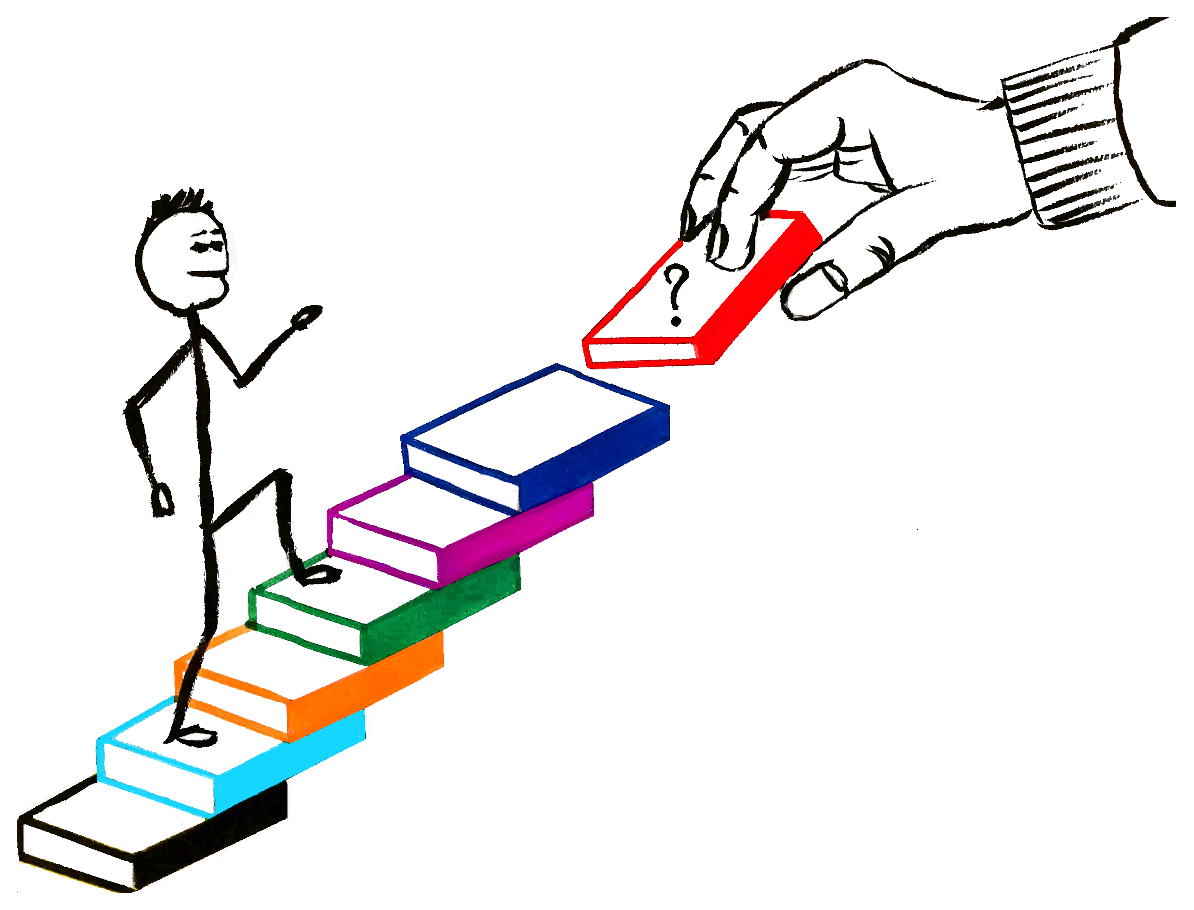
\includegraphics[height=6cm]{escaliers_Nath}}
      \rput[lb](8,1){\parbox{6.5cm}{\it Un escalier compte moins de 100 marches. \\
   Si on le monte 3 par 3, 4 par 4, ou encore 5 par 5, à chaque fois on arrive exactement sur la dernière marche.}}
         \end{pspicture}
\partie[les questions]
   \begin{enumerate}
      \item Combien y a-t-il de marches à cet escalier ?
      \item Arriverait-on exactement sur la dernière marche de cet escalier si on le montait :
      \begin{enumerate}
         \item en sautant 6 marches à la fois ?
         \item en sautant 8 marches à la fois ?
         \item en sautant 5 marches, puis 7, à nouveau 5, puis 7, et ainsi de suite ?
         \item en sautant 3 marches, puis 4, à nouveau 3, puis 4, et ainsi de suite ? et en sautant d'abord 4 marches ?
      \end{enumerate}
   \end{enumerate}
\partie[la narration de recherche]
 
